\section{圆周运动和一般曲线运动}

\subsection{切向加速度和法向加速度}

\subsubsection{自然坐标系}

{在圆周轨迹上任意一点P，沿轨迹在P点的切线方向建立一坐标轴，该方向上的单位矢量用$\mathbf{e}_t$表示，另一坐标轴沿该点轨迹的法线并指向曲线凹侧，相应单位矢量用用$\mathbf{e} _n$表示，这种坐标系就叫做自然坐标系。}

\hspace*{\fill}

{优点：坐标轴随动点位置的变化而变化，且切向速度与法向速度始终与两坐标轴同向，相互垂直，不产生联动影响。}


\begin{figure}[h]
	\centering
	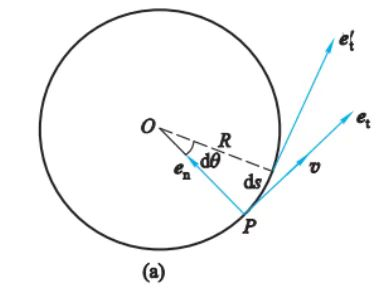
\includegraphics[width=0.3\linewidth]{images/naturesys.jpg}
	\caption{自然坐标系}
\end{figure}

\subsubsection{加速度}
\begin{figure}[h]
	\centering
	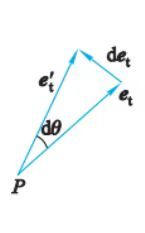
\includegraphics[width=0.25\linewidth]{images/nature.jpg}

\end{figure}

	{在极短时间内，$\mathbf{e}_t$与$\mathrm{d}\mathbf{e}_t$可视为相互垂直，则$\mathrm{d}\mathbf{e}_t$方向与$\mathbf{e}_n$相同,在大小上，$|\mathrm{d}\mathbf{e}_t|$=$|\mathrm{d}\theta|$。}
	
	$\mathbf{v}=v\mathbf{e}_t$
	
	\hspace*{\fill}
	
	$\mathbf{a}=\dfrac{\mathrm{d}\mathbf{v}}{\mathrm{d}t}=\dfrac{\mathrm{d}}{\mathrm{d}t}(v\mathbf{e}_t)=\dfrac{\mathrm{d}v}{\mathrm{d}t}\mathbf{e}_t+v\dfrac{\mathrm{d}\mathbf{e}_t}{\mathrm{d}t}$
	
	\vspace{12pt}
	
	$\mathrm{d}\mathbf{e}_t$=$\mathrm{d}\theta\mathbf{e} _n$
	
	\vspace{12pt}
	
	{对于$\frac{\mathrm{d}\mathbf{e}_t}{\mathrm{d}t}$：}

	$\dfrac{\mathrm{d}\mathbf{e}_t}{\mathrm{d}t}=\dfrac{\mathrm{d}\theta}{\mathrm{d}t}\mathbf{e}_n=\omega\mathbf{e} _n=\frac{v}{R}\mathbf{e} _n$
	
	{则$\mathbf{a}=\dfrac{\mathrm{d}\mathbf{v}}{\mathrm{d}t}\mathbf{e}_t+\dfrac{v^2}{R}\mathbf{e} _n$}
	
	{切向加速度$\mathbf{a}_t=\dfrac{\mathrm{d}\mathbf{v}}{\mathrm{d}t}\mathbf{e}_t$,表示速率变化快慢}
	
	{法向加速度$\mathbf{a}_n=\dfrac{v^2}{R}\mathbf{e} _n$，表示方向变化快慢}


\subsection{圆周运动的角量描述}

{角位置$\theta$}

{角位移$\Delta\theta$}

{角速度$\omega=\lim_{{\Delta}t\rightarrow0}\dfrac{\Delta\theta}{\Delta t}=\dfrac{\mathrm{d}\theta}{\mathrm{d}t}$}

{角加速度$\mathbf{a}=\lim_{{\Delta}t\rightarrow0}\dfrac{\Delta\omega}{\Delta t}=\dfrac{\mathrm{d}\omega}{\mathrm{d}t}=\dfrac{\mathrm{d}^2\theta}{\mathrm{d}t^2}$}

{匀变速圆周运动(类比匀加速直线运动)}

{$\omega=\omega_0 +\mathbf{a}t$}

{$\varphi=\varphi_0 +\omega_0 t+\frac{1}{2}\mathbf{a}t^2$}

{$\omega^2-{\omega_0}^2=2\mathbf{a}(\varphi-\varphi_0)$}


\subsection{角量和线量的关系}
\subsubsection{相关线量和角量}
以下是圆周运动中的相关线量和角量。

线量：速度$\mathbf{v}$、加速度$\mathbf{a}$

角量：角速度$\omega$、角加速度$\alpha$

\subsubsection{线量和角量的关系}
设圆的半径为$R$。

\begin{figure}[h]
	\centering
	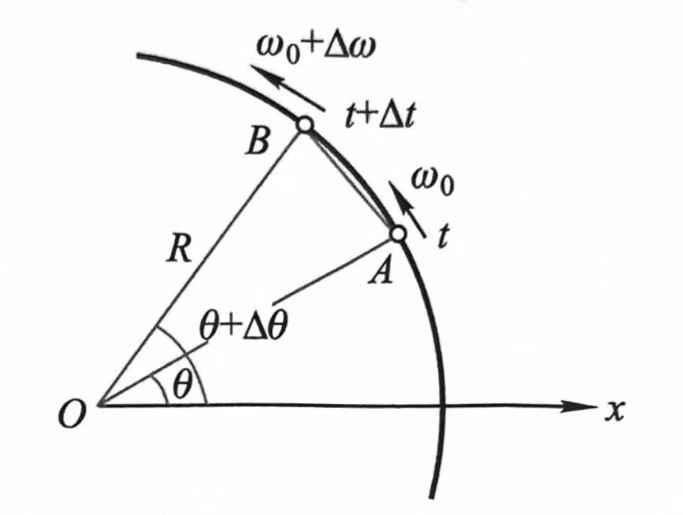
\includegraphics[width=0.5\textwidth]{images/ang-lin.jpg}
	\caption{线量和角量间的关系推导}
\end{figure}

\textbf{线速度和角速度：}
\begin{equation}
	v=R\omega
\end{equation}

\textbf{加速度和角加速度：}

切向加速度
\begin{equation}
	a_t=R\alpha
\end{equation}

法向加速度
\begin{equation}
	a_n=\frac{v^2}{R}=v\omega=R\omega ^2
\end{equation}

\subsubsection{一般平面曲线运动中的加速度}
质点沿轨迹作一般曲线运动时，上面讨论的有关变速圆周运动中加速度的结果也都是适用的。

但法向加速度式中的R要用曲线在该点处的曲率半径$\rho$来代替。

即
\begin{equation}
	\mathbf{a_t}=\frac{\mathrm{d}v}{\mathrm{d}t}\mathbf{e_t}
\end{equation}
\begin{equation}
	\mathbf{a_n}=\frac{v^2}{\rho}\mathbf{e_n}
\end{equation}
\begin{equation}
	\mathbf{a}=\mathbf{a_t}+\mathbf{a_n}=\frac{\mathrm{d}v}{\mathrm{d}t}\mathbf{e_t}+\frac{v^2}{\rho}\mathbf{e_n}
\end{equation}

法向加速度$a_n$处处指向曲率中心。 

一般来说，曲线上各点的曲率中心和曲率半径是逐点变化的。

\begin{figure}[h]
	\centering
	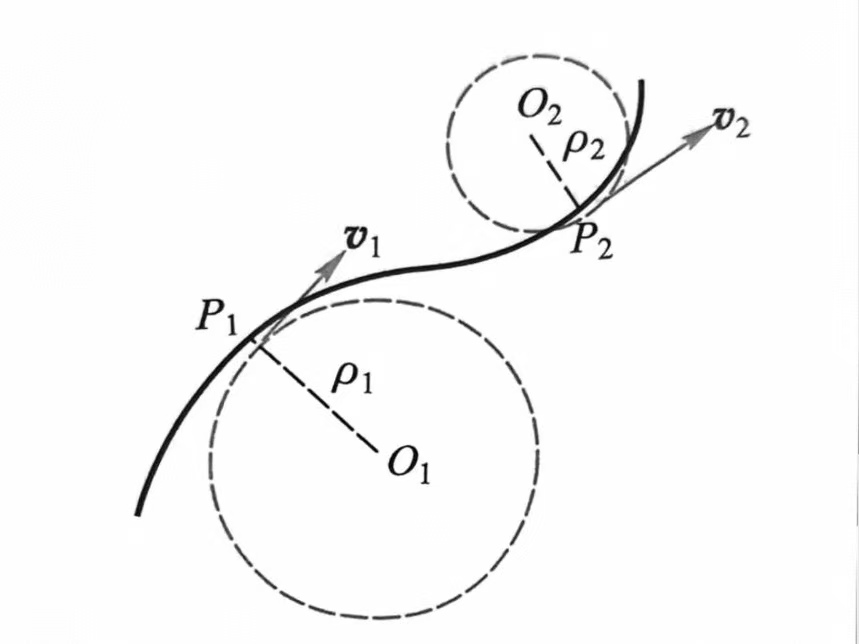
\includegraphics[width=0.5\textwidth]{images/rho.jpg}
	\caption{曲率圆和曲率半径}
\end{figure}
